\documentclass[fleqn,letterpaper,12pt,printwatermark=false]{memoir}
% memoir commands to define the text block geometry
\setulmarginsandblock{0.5in}{*}{*}
\setlrmarginsandblock{0.5in}{*}{*}
% put "extra" vertical space at the bottom of a page
\raggedbottom 

\usepackage{amsmath}
\usepackage{xparse} % for NewDocumentCommand et al.
\usepackage{enumitem}
\usepackage{transparent} % for \transparent, which I use in the watermark
\usepackage[slantedGreek]{mathpazo} \usepackage{helvet} % use Palatino et al.
\usepackage{booktabs} % prettier tables

\usepackage[]{xwatermark}
\newwatermark*[
    allpages,
    color=red!30,angle=45,
    scale=4,
    xpos=-10, ypos=0
]{%
    \transparent{0.4}dhasan example%
}

\usepackage{dashundergaps} % for \gap
\dashundergapssetup{
    teacher-mode=true, % set to true to show answers 
    gap-format=underline,
    teacher-gap-format=underline,
    gap-font={\sffamily},
    gap-numbers=true,
    gap-widen=true,
    gap-extend-percent=150, % note: making this too big might create errors
    gap-number-format=\,\textsuperscript{\normalfont(\thegapnumber)},
}

\usepackage{tcolorbox}
\tcbuselibrary{skins}
\tcbuselibrary{raster}

\usepackage{pgfplots}
\pgfplotsset{compat=newest}

% ---------------------DOCUMENT------------------------------
\begin{document}

\newcommand{\myClassName}{Pre-AP Algebra 2}
\newcommand{\myUnitNumber}{1}
\newcommand{\myUnitTitle}{Introduction to Functions}
\newcommand{\myLessonNumber}{99}
\newcommand{\myLessonTitle}{Sketching Inverses}

\copypagestyle{myPagestyle}{empty}


\newcommand{\myFooterSize}{\footnotesize}
\makeoddfoot{myPagestyle}{\myFooterSize\myClassName}{\myFooterSize\thepage\,of\,\pageref*{xwmlastpage}}{\myFooterSize\myLessonTitle}
\makeevenfoot{myPagestyle}{\myFooterSize\myLessonTitle}{\myFooterSize{\thepage{}~of~\pageref*{xwmlastpage}}}{\myFooterSize\myClassName}

%
% A command to change the appearance of the cognitive verb 
% in the objectives.
%
\newcommand{\myCognitiveVerb}[1]{\textcolor{blue}{\textbf{#1}}}

%
% Font styling commands (so I can change them in a single place)
%
\NewDocumentCommand{\myUnitLessonNumberFont}{}{\sffamily\bfseries\HUGE}
\NewDocumentCommand{\myUnitTitleFont}{}{\sffamily\large}
\NewDocumentCommand{\myLessonTitleFont}{}{\sffamily\bfseries\huge}
\NewDocumentCommand{\myHeadingFont}{}{\sffamily\bfseries\Large}


%
% #1 is the fill-in text
%
\NewDocumentCommand{\myFillInBlank}{m}{%
    \,%
    \gap[u]{#1}%
    \,%
}


% Definition for the LESSON HEADER + OBJECTIVES
%
\newenvironment{myNotesHeader}{
    \begin{flushleft}
        {\myUnitLessonNumberFont{\myUnitNumber.\myLessonNumber}}
        \hfill\;\;
        \begin{minipage}[b]{0.75\textwidth}
            \begin{flushright}
                {\myUnitTitleFont{}Unit \myUnitNumber\,\,\,\myUnitTitle}\\ \vspace{0.75em}
                {\myLessonTitleFont\myLessonTitle}
            \end{flushright}
        \end{minipage}
        \hrule
    \end{flushleft}
    \noindent{\myHeadingFont Objectives:}
    \begin{enumerate}[label=\arabic*)]
}{
    \end{enumerate}
}


% Definitions related to the VOCABULARY TABLE
%
\newenvironment{myVocabulary}{
    {\noindent{\myHeadingFont Vocabulary:}}\vspace{1em}

    \begin{tabular}{ll}
        \toprule
            \emph{word} & \emph{meaning} \\ 
        \midrule
}{
    \bottomrule
    \end{tabular}
    \vspace{1em}
}

\newcommand{\myVocabularyWord}[2]{%
{\textcolor{blue}{\textbf{#1}}} & #2 \\
}


% Definitions related to an INTRODUCTION
%
\newenvironment{myLesson}{
    {\noindent{\myHeadingFont Lesson:}}\vspace{1em}

    \begin{adjustwidth}{2em}{0pt}
    \begin{itemize}
}{
    \end{itemize}
    \end{adjustwidth}
    \vspace{1em}
}


% Definition related to KEY CONCEPTS
%
% #1 : the key concept (which appears as a tcolorbox title)
%
\NewDocumentEnvironment{myKeyConcepts}{ O{Key Concepts:} }{
    \begin{tcolorbox}[
        title=#1, fonttitle=\myHeadingFont,
        coltitle=black, 
        colbacktitle=black!25!yellow, 
        colframe=black!50!yellow,
        colback=white!70!yellow,
        boxrule=2pt, 
        ]
}{
    \end{tcolorbox}
}


% Definition related to EXAMPLES

% #1 Optional example number 
% #2 A statement of the example problem.
% #3 How much empty vertical space to leave for the example box.
%
\NewDocumentCommand{\myExample}{omm}{%
    \begin{tcolorbox}[
        enhanced,
        sharp corners, 
        colback=white,
        boxrule=0pt,
        borderline={0.5pt}{0pt}{black,dashed},
        ]
        {\myHeadingFont Example\IfValueT{#1}{{ #1}}:}
        #2
        \tcblower
        \vspace{#3}
    \end{tcolorbox}
}

% #1 Optional example number 
% #2 A statement of the example problem.
%
\NewDocumentEnvironment{myExampleForTikzGraphs}{om}{%
    \begin{tcolorbox}[
        enhanced,
        sharp corners, 
        colback=white,
        boxrule=0pt,
        borderline={0.5pt}{0pt}{black,dashed},
        ]
        {\myHeadingFont Example\IfValueT{#1}{{ #1}}:}
        #2
        \tcblower
        \begin{center}
}
% user would insert 
% \begin{tikzpicture}\begin{axis}...\end{axis}\end{tikzpicture}
{
        \end{center}
    \end{tcolorbox}
}


% Definitions related to PROBLEMS

% A counter to number the problems in the guided notes.
\newcounter{MyProblemCounter}
\setcounter{MyProblemCounter}{1}
\newcommand{\useMyProblemCounter}{\theMyProblemCounter\stepcounter{MyProblemCounter}}

% an environment for two adjacent problems
%
% #1 : directions for all the problems
% #2 : vertical height of the problem boxes
% #3 : details for problem 1
% #4 : details for problem 2
%
\newenvironment{myProblems2}[4]{%
    \noindent
    {\myHeadingFont Practice:}\hspace{0.5em}#1\nopagebreak%
    \begin{tcbraster}[%
        raster equal height,%
        raster columns=2,%
        raster column skip=0.5mm,%
        raster row skip=0.5mm,%
        raster every box/.style={%
            enhanced,%
            sharp corners,%
            colback=white,%
            coltitle=black, colbacktitle=black!10!white,%
            boxrule=0pt, borderline={0.5pt}{0pt}{black},%
            title={\texttt\useMyProblemCounter},%
            },%
        ]%
        \begin{tcolorbox}[attach boxed title to top left]
            #3
            \tcblower\vspace{#2}
        \end{tcolorbox}
        \begin{tcolorbox}[attach boxed title to top right]
            #4
            \tcblower
        \end{tcolorbox}%
}{%
    \end{tcbraster}
}

% an environment for 4 adjacent problems
%
% #1 : directions for all the problems
% #2 : vertical height of the problem boxes
% #3 : details for problem 1
% #4 : details for problem 2
% #5 : details for problem 3
% #6 : details for problem 4
%
\newenvironment{myProblems4}[6]{%
    \noindent
    \textbf{\myHeadingFont Practice:}\hspace{0.5em}#1\nopagebreak%
    \begin{tcbraster}[%
        raster equal height,%
        raster columns=2,%
        raster column skip=0.5mm,%
        raster row skip=0.5mm,%
        raster every box/.style={%
            enhanced,%
            sharp corners,%
            colback=white,%
            coltitle=black, colbacktitle=black!10!white,%
            boxrule=0pt, borderline={0.5pt}{0pt}{black},%
            title={\texttt\useMyProblemCounter},%
            },%
        ]%
        \begin{tcolorbox}[attach boxed title to top left]
            #3
            \tcblower\vspace{#2}
        \end{tcolorbox}
        \begin{tcolorbox}[attach boxed title to top right]
            #4
            \tcblower
        \end{tcolorbox}%
        \begin{tcolorbox}[attach boxed title to bottom left]
            #5
            \tcblower
        \end{tcolorbox}%
        \begin{tcolorbox}[attach boxed title to bottom right]
            #6
            \tcblower
        \end{tcolorbox}%
}{%
    \end{tcbraster}
}
\pagestyle{myPagestyle}

\checkandfixthelayout
\setlist{labelindent=\parindent,leftmargin=*,itemsep=0.025em,label=$\circ$}

% ---------------------LESSON------------------------------
\begin{myNotesHeader}
    \item \myCognitiveVerb{sketch} the graph of the inverse of a relation given its graph
\end{myNotesHeader}

\begin{myVocabulary}
    \myVocabularyWord{sketch}
        {
            draw something quickly without being perfect
        }
    \myVocabularyWord{graph of a relation}
        {
            a plot of the relation on a 2-D grid (eg, $x$-$y$ axes)
        }
    \myVocabularyWord{inverse functions}
        {
            two functions that ``undo'' each other
        }
    \myVocabularyWord{ordered pair}
        {
            two numbers in parentheses, (1,4) or (-3,19)
        }
\end{myVocabulary}

\begin{myLesson}
    \item 
    You know how to find the inverse of a given function
    algebraically (using {\bfseries equations}).
    \item
    Now you'll learn how to sketch the \emph{graph} of an inverse function.
    \item 
    This involves reflections which you learned in Geometry.
    \item
    You will \emph{swap} the coordinates of the points (eg, swap $x$ and $y$),
    geometrically (by {\bfseries drawing}).
\end{myLesson}

% ---------------------CONCEPT 1------------------------------
\begin{myKeyConcepts}[To sketch the inverse of a relation given its graph as a bunch of points\dots]
    Follow these steps:
    \setlist{labelindent=\parindent,itemsep=0.4em}
    \begin{enumerate}
        \item Find the ($x$,$y$) pair of each point 
        in the graph of original relation.
        \item For each of those ordered pairs, 
        swap the $x$ and $y$ coordinates.
        This will give you a new pair with the numbers reversed.
        \item Plot each of the new ordered pairs on the graph.
        Use a \emph{different symbol} for these new points.
    \end{enumerate}
    The graph of the inverse function is all those new points 
    that you just plotted. But the new points will be the reflection 
    of the old points across the diagonal line $y=x$.
\end{myKeyConcepts}

\begin{myExampleForTikzGraphs}[1]{
    Sketch the inverse of the relation shown in this graph.
    (Notice in this example, you have to draw in the diagonal line yourself.)
}
    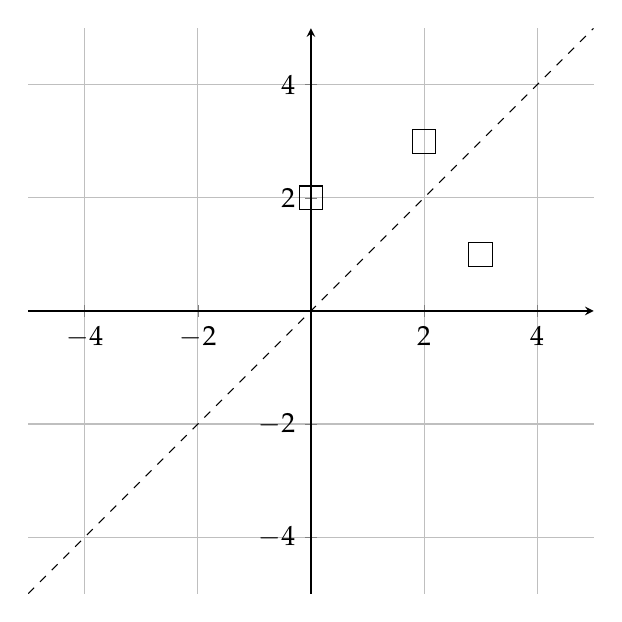
\begin{tikzpicture}
        \begin{axis}[
            width=4in,
            grid=both,
            axis x line = middle,axis y line = middle,
            axis equal image,
            xtick distance = 2, ytick distance = 2,
            ]
            \addplot[no marks,dashed]{x};
            \addplot[
                only marks,
                mark=square,
                mark size = 0.15cm,
                ] coordinates { (0,2) (2,3) (3,1) };
        \end{axis}
    \end{tikzpicture}
\end{myExampleForTikzGraphs}

\begin{myExampleForTikzGraphs}[2]{
    Sketch the inverse of the relation shown in this graph.
    (Notice in this example, you have to draw in the diagonal line yourself.)
}
    \begin{tikzpicture}
        \begin{axis}[
            width=4in,
            grid=both,
            axis x line = middle,axis y line = middle,
            axis equal image,
            xtick distance = 2, ytick distance = 2,
            ]
            \addplot[
                only marks,
                mark=square,
                mark size = 0.15cm,
                ] coordinates { (-2,3) (4,-2) (2,5) (2,-2) };
        \end{axis}
    \end{tikzpicture}
\end{myExampleForTikzGraphs}

% ---------------------CONCEPT 2------------------------------
\begin{myKeyConcepts}[To sketch the inverse of a relation given its graph as a curve\dots]
    Follow these steps:
    \setlist{labelindent=\parindent,itemsep=0.4em}
    \begin{enumerate}
        \item Draw several points on the curve.
        \item Find the ($x$,$y$) ordered pair of each of your points.
        \item For each of those ordered pairs, 
        swap the $x$ and $y$ coordinates.
        This will give you a bunch of new ordered pairs with the numbers reversed.
        \item Plot each of the new ordered pairs on the graph.
        Use a \emph{different symbol} for these new points.
        \item Sketch a curve going through the new points, 
        doing your best to make the curve the \emph{mirror image} 
        of the original curve across the diagonal line, $y=x$.
    \end{enumerate}
    The curve you sketched is the graph of the inverse of the original function.
\end{myKeyConcepts}

\begin{myExampleForTikzGraphs}[1]{foo bar baz}
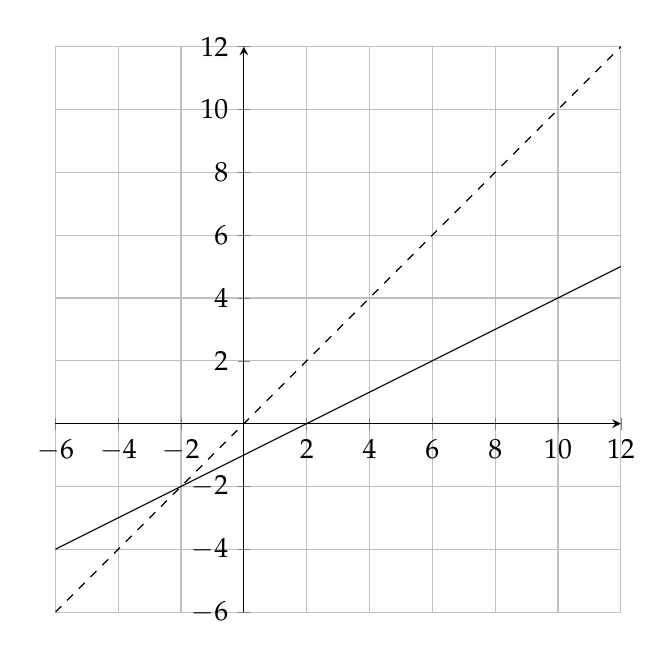
\begin{tikzpicture}
    \begin{axis}[
        width=4in,
        grid=both,
        axis x line = middle,axis y line = middle,
        axis equal image,
        xtick distance = 2, ytick distance = 2,
        ]
        \addplot[no marks,dashed,domain=-6:12]{x};
        \addplot[no marks,solid, domain=-6:12]{(1/2)*x - (1)};
    \end{axis}
\end{tikzpicture}
\end{myExampleForTikzGraphs}

% ---------------------PROBLEMS------------------------------
% \begin{myProblems2}%
%     {Factor the following monomials into prime factors.}%
%     {2in}%
%     %
%     {\( 32x^2 \)}
%     {\( 8 x^3y^2z \)}
% \end{myProblems2}
  


\end{document}